% id: 0140
% book: 쎈 중3-2 수학 · 01 삼각비
% section: C단계 만점 도전하기
% figure: tikz:fig-0140
% answer: $42^\circ$
% answer_source: 해설
% variant_level: 0 (원본 전사)
% 이 파일은 build.mjs 가 items.json 에서 만든다. 고칠 때는 items.json 을 고친다.
\smash{\raisebox{1.5mm}{\dmkichul{쎈 중3-2 수학 0140번 · 29쪽}}}
\noindent\begin{minipage}[t]{0.58\linewidth}\vspace{0pt}\raggedright 오른쪽 그림과 같이 모선~$\pt{AB}$의 길이가 $50\,\mathrm{cm}$이고 밑면의 반지름의 길이가 $37\,\mathrm{cm}$인 원뿔이 있다. 이 원뿔의 밑면의 중심을 $\pt{O}$라 할 때, $\angle\pt{ABO}$의 크기를 다음 삼각비의 표를 이용하여 구하시오.\end{minipage}\hfill\begin{minipage}[t]{0.4\linewidth}\vspace{0pt}\centering \resizebox{\ifdim\width>\linewidth\linewidth\else\width\fi}{!}{% 0140(본책 29쪽) — 모선 AB=50 cm·밑면 반지름 37 cm 인 원뿔, 밑면의 중심 O, 높이 AO(직각 표시). 라벨 A·O·B·50 cm(파선 호)·37 cm. 스캔 삽화(입체)를 TikZ 로 다시 그림. 답(∠ABO)은 적지 않는다.
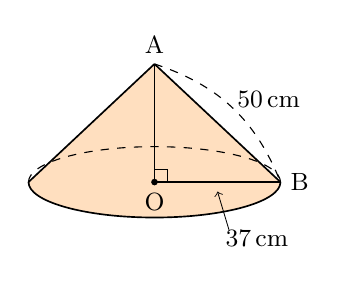
\begin{tikzpicture}[line width=0.6pt]
  \coordinate (A) at (0,1.5); \coordinate (O) at (0,0); \coordinate (B) at (1.6,0); \coordinate (L) at (-1.6,0);
  \fill[orange!25] (L) -- (A) -- (B) arc[start angle=0, end angle=-180, x radius=1.6, y radius=0.45] -- cycle;
  \draw (A) -- (B);
  \draw (A) -- (L);
  \draw (B) arc[start angle=0, end angle=-180, x radius=1.6, y radius=0.45];
  \draw[dashed, line width=0.4pt] (L) arc[start angle=180, end angle=0, x radius=1.6, y radius=0.45];
  \draw (A) -- (O);
  \draw (O) -- (B);
  \fill (O) circle (1.2pt);
  % 직각 표시(O)
  \draw[line width=0.4pt] (0,0.16) -- (0.16,0.16) -- (0.16,0);
  % AB=50 cm(파선 호)
  \draw[dashed, line width=0.4pt] (A) to[bend left=25] (B);
  \node[font=\small] at (1.45,1.05) {$50\,\mathrm{cm}$};
  % 반지름 37 cm
  \node[font=\small] at (1.3,-0.72) {$37\,\mathrm{cm}$};
  \draw[line width=0.3pt, ->] (0.95,-0.62) -- (0.8,-0.12);
  \node[font=\small, above] at (A) {A};
  \node[font=\small, below] at (0,-0.02) {O};
  \node[font=\small, right] at (B) {B};
\end{tikzpicture}
}\end{minipage}\par
\par\smallskip\begin{center}\resizebox{\ifdim\width>\linewidth\linewidth\else\width\fi}{!}{% 0140(본책 29쪽) — 42°~44° 삼각비의 표(figure_extra). 원문 표를 tabular 로 옮김(값 그대로).
{\renewcommand{\arraystretch}{1.45}\small
\begin{tabular}{|c|c|c|c|}
\hline
각도 & 사인(sin) & 코사인(cos) & 탄젠트(tan) \\ \hline
$42^\circ$ & $0.67$ & $0.74$ & $0.90$ \\ \hline
$43^\circ$ & $0.68$ & $0.73$ & $0.93$ \\ \hline
$44^\circ$ & $0.69$ & $0.72$ & $0.97$ \\ \hline
\end{tabular}}
}\end{center}
